\section{Existing Backends}

\begin{frame}[fragile]{Agda Architecture}
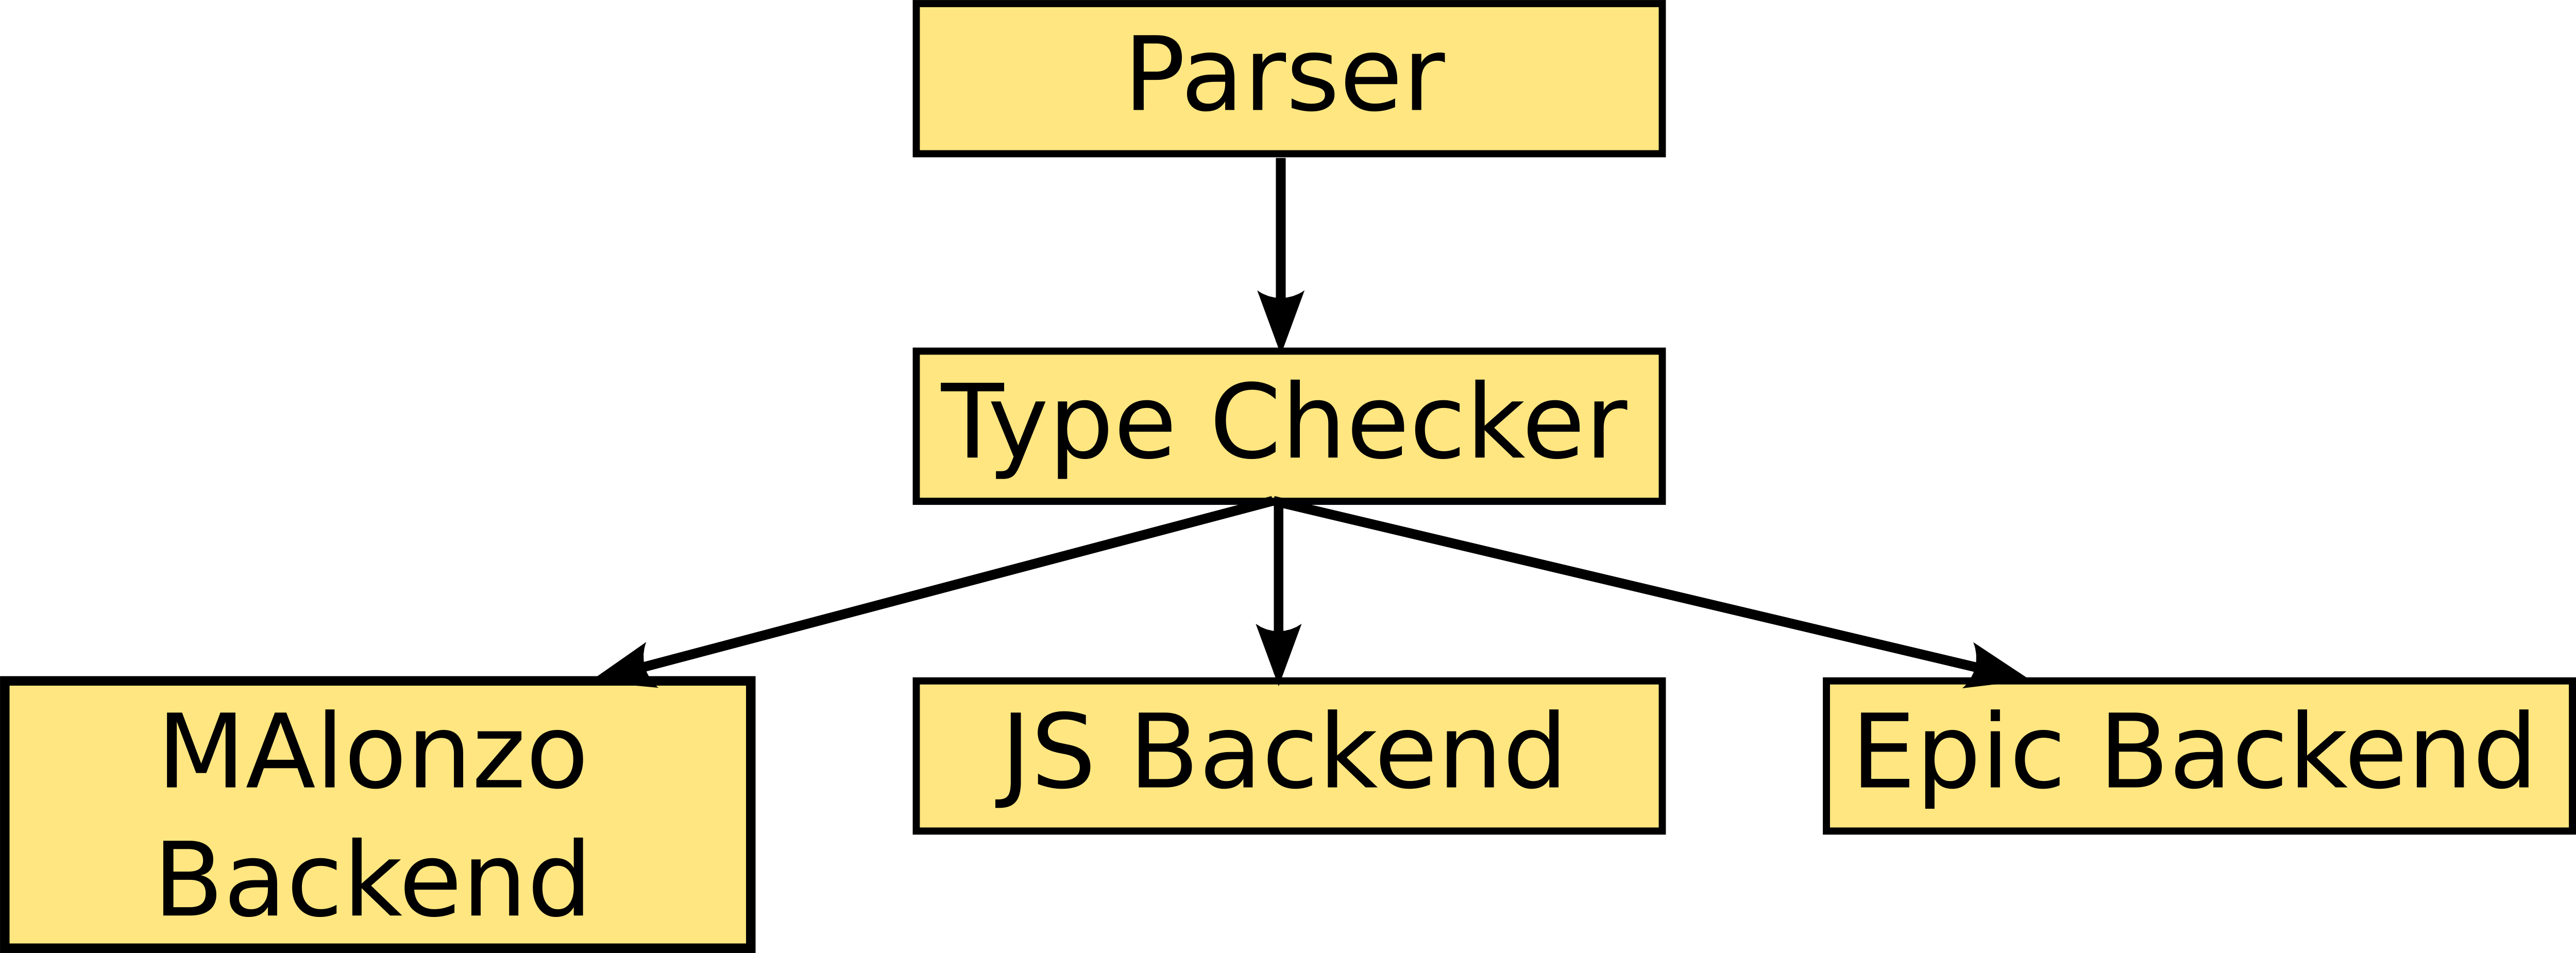
\includegraphics[width=250px]{agda-arch.png}
\end{frame}

\subsection{MAlonzo backend}
\begin{frame}{MAlonzo backend}
\begin{itemize}
\item Targets Haskell
\item Maintained
\item Relies on GHC for optimizations
\end{itemize}
\end{frame}


\begin{frame}{MAlonzo - FFI}
\begin{itemize}
\item Provides simple FFI to haskell
\item Very limited
  \begin{itemize}
    \item No class support
    \item Can't export Agda datatypes
    \item Not automatic
  \end{itemize}
\end{itemize}
\end{frame}

\begin{frame}[fragile]{MAlonzo - FFI}
\begin{code}%
\>\AgdaSymbol{\{-\#} \AgdaKeyword{IMPORT} Data.List \AgdaSymbol{\#-\}}\<%
\\
%
\\
\>\AgdaKeyword{data} \AgdaDatatype{List} \AgdaSymbol{:} \AgdaSymbol{(}\AgdaBound{A} \AgdaSymbol{:} \AgdaPrimitiveType{Set}\AgdaSymbol{)} \AgdaSymbol{->} \AgdaPrimitiveType{Set} \AgdaKeyword{where}\<%
\\
\>[0]\AgdaIndent{2}{}\<[2]%
\>[2]\AgdaInductiveConstructor{nil} \AgdaSymbol{:} \AgdaSymbol{∀} \AgdaSymbol{\{}\AgdaBound{A}\AgdaSymbol{\}} \AgdaSymbol{→} \AgdaDatatype{List} \AgdaBound{A}\<%
\\
\>[0]\AgdaIndent{2}{}\<[2]%
\>[2]\AgdaInductiveConstructor{cons} \AgdaSymbol{:} \AgdaSymbol{∀} \AgdaSymbol{\{}\AgdaBound{A}\AgdaSymbol{\}} \AgdaSymbol{→} \AgdaBound{A} \AgdaSymbol{→} \AgdaDatatype{List} \AgdaBound{A} \AgdaSymbol{→} \AgdaDatatype{List} \AgdaBound{A}\<%
\\
\>\AgdaSymbol{\{-\#} \AgdaKeyword{COMPILED\_DATA} \AgdaDatatype{List} Data.List nil cons \AgdaSymbol{\#-\}}\<%
\\
%
\\
\>\AgdaKeyword{postulate}\<%
\\
\>[0]\AgdaIndent{2}{}\<[2]%
\>[2]\AgdaPostulate{head} \AgdaSymbol{:} \AgdaSymbol{∀} \AgdaSymbol{\{}\AgdaBound{A}\AgdaSymbol{\}} \AgdaSymbol{→} \AgdaDatatype{List} \AgdaBound{A} \AgdaSymbol{->} \AgdaBound{A}\<%
\\
\>\AgdaSymbol{\{-\#} \AgdaKeyword{COMPILED} \AgdaPostulate{head} Data.List.head \AgdaSymbol{\#-\}}\<%
\\
\>\<%
\end{code}
\end{frame}

\begin{frame}[fragile]{MAlonzo - Code Generation}
\begin{code}%
\>\AgdaFunction{vecToStr} \AgdaSymbol{:} \AgdaSymbol{∀} \AgdaSymbol{\{}\AgdaBound{A} \AgdaBound{m}\AgdaSymbol{\}} \AgdaSymbol{→} \AgdaSymbol{(}\AgdaBound{A} \AgdaSymbol{→} \AgdaPostulate{String}\AgdaSymbol{)}\<%
\\
\>[2]\AgdaIndent{4}{}\<[4]%
\>[4]\AgdaSymbol{→} \AgdaDatatype{Vec} \AgdaBound{A} \AgdaBound{m} \AgdaSymbol{→} \AgdaPostulate{String}\<%
\\
\>\AgdaFunction{vecToStr} \AgdaBound{f} \AgdaInductiveConstructor{[]} \AgdaSymbol{=} \AgdaString{""}\<%
\\
\>\AgdaFunction{vecToStr} \AgdaBound{f} \AgdaSymbol{(}\AgdaBound{x} \AgdaInductiveConstructor{::} \AgdaBound{xs}\AgdaSymbol{)} \AgdaSymbol{=} \AgdaString{", "} \AgdaFunction{++} \AgdaSymbol{((}\AgdaBound{f} \AgdaBound{x}\AgdaSymbol{)}\<%
\\
\>[2]\AgdaIndent{4}{}\<[4]%
\>[4]\AgdaFunction{++} \AgdaSymbol{(}\AgdaFunction{vecToStr} \AgdaBound{f} \AgdaBound{xs}\AgdaSymbol{))}\<%
\end{code}

%\ExecuteMetaData[src/agda/latex/HelloDatHS.tex]{vecToStr}

%\input{src/agda/latex/HelloDat_HS.tex}
\end{frame}

\begin{frame}[fragile]{MAlonzo - Code Generation}
\begin{lstlisting}[language=Haskell,basicstyle=\scriptsize]
d55 v0 v1 v2 v3
  = MAlonzo.RTE.§\colorbox{yellow}{mazCoerce}§
      (d_1_55 (MAlonzo.RTE.§\colorbox{yellow}{mazCoerce}§ v0)
         (MAlonzo.RTE.§\colorbox{yellow}{mazCoerce}§ v1)
         (MAlonzo.RTE.§\colorbox{yellow}{mazCoerce}§ v2)
         (MAlonzo.RTE.§\colorbox{yellow}{mazCoerce}§ v3))
  where d_1_55 v0 v1 v2 (C51 v3 v4 v5)
          = MAlonzo.RTE.§\colorbox{yellow}{mazCoerce}§
              (d33 (MAlonzo.RTE.§\colorbox{yellow}{mazCoerce}§ ", ")
                 (MAlonzo.RTE.§\colorbox{yellow}{mazCoerce}§
  (d33 (MAlonzo.RTE.§\colorbox{yellow}{mazCoerce}§ (v2 (MAlonzo.RTE.§\colorbox{yellow}{mazCoerce}§ v4)))
     (MAlonzo.RTE.§\colorbox{yellow}{mazCoerce}§
        (d55 (MAlonzo.RTE.§\colorbox{yellow}{mazCoerce}§ v0) (MAlonzo.RTE.§\colorbox{yellow}{mazCoerce}§ v3)
           (MAlonzo.RTE.§\colorbox{yellow}{mazCoerce}§ v2)
           (MAlonzo.RTE.§\colorbox{yellow}{mazCoerce}§ v5))))))
        d_1_55 v0 v1 v2 v3 = MAlonzo.RTE.mazIncompleteMatch name55
\end{lstlisting}
\end{frame}

\begin{frame}{MAlonzo - Summary}
\begin{itemize}
  \item Produces 'strange' haskell code
  \item Can lead to size blow-up
  \begin {itemize}
    \item 84 lines Agda - 250'000 lines Haskell - 300 Mb executable (CITE)
  \end{itemize}
\end{itemize}
\end{frame}

\subsection{JS backend}
\begin{frame}{JS backend}
\begin{itemize}
\item Targets Javascript
\item Not maintained
\item Very similar to MAlonzo
\end{itemize}
\end{frame}

\subsection{Epic backend}
\begin{frame}{Epic backend}
\begin{itemize}
\item Targets Epic
\item Not maintained
\end{itemize}
\end{frame}

\begin{frame}{Epic}
\begin{itemize}
\item Untyped-lambda calculus with some extensions
\item Intended as building block for compilers
\item Also not maintained
\end{itemize}
\end{frame}

\begin{frame}[fragile]{Epic Language}
\begin{tabular}{c r l}
\hline
\multicolumn{3}{l}{Epic Language} \\
\hline
$t$ & $::=$ & $x$            \\
& \textbar & $t$ $\vec{t}$            \\
& \textbar & $\lambda x \rightarrow t$  \\
& \textbar & Con $i$ $\vec{t}$         \\
& \textbar & if $t$ then $t$ else $t$  \\
& \textbar & case $t$ of $\vec{alt}$   \\
& \textbar & let $x$ = $t$ in $t$      \\
& &                                    \\
& \textbar & lazy $t$                  \\
& \textbar & $t$ $!$ $i$               \\
& \textbar & $i$                       
%\\
%$alt$ & ::= & Con $i$ $\vec{x}$ $\rightarrow$ $t$     \\
%& \textbar & $i$ $\rightarrow$ $t$                    \\
%& \textbar & default $\rightarrow$ $t$               
\end{tabular}
\end{frame}

\begin{frame}[fragile]{Epic - Nat Optimizations}
\begin{itemize}
\item \begin{code}%
\>\AgdaKeyword{data} \AgdaDatatype{Nat} \AgdaSymbol{:} \AgdaPrimitiveType{Set} \AgdaKeyword{where}\<%
\\
\>[0]\AgdaIndent{2}{}\<[2]%
\>[2]\AgdaInductiveConstructor{zero} \AgdaSymbol{:} \AgdaDatatype{Nat}\<%
\\
\>[0]\AgdaIndent{2}{}\<[2]%
\>[2]\AgdaInductiveConstructor{succ} \AgdaSymbol{:} \AgdaDatatype{Nat} \AgdaSymbol{->} \AgdaDatatype{Nat}\<%
\\
\>\AgdaSymbol{\{-\#} \AgdaKeyword{BUILTIN} NATURAL \AgdaDatatype{Nat} \AgdaSymbol{\#-\}}\<%
\\
\>\<%
\end{code}
\item Naive translation is horribly slow
\item Can be transformed into arbitrary precision Integers
\item Automatic detection of Nat-like datatypes
\end{itemize}
\end{frame}


\pgfplotsset{compat=1.8}
\pgfplotstableread{
paradigm position time
{MAlonzo}     1       618
{MAlonzo with Pragma}   2   217
{Epic}        3     269
}\mytable

\begin{frame}{Nat Performance}
\begin{tikzpicture}[scale=.75]
        \begin{axis}[%
          ybar, bar width=1.5cm,%
          xmin=0.5,xmax=3.5, xtick=data,ymin=0,%
          xticklabels from table={\mytable}{paradigm},%
          xticklabel style={rotate=45,anchor=north east,inner sep=0mm},%
          ylabel={\Large Time (ms)}, ylabel near ticks]
          \addplot table [x=position,y=time] {\mytable};
        \end{axis}
\end{tikzpicture}
\end{frame}


\begin{frame}{Comparison}
\end{frame}
